\documentclass[12pt,addpoints,answers]{evalua}
\grado{3$^\circ$ de Secundaria}
\cicloescolar{2023-2024}
\materia{Matemáticas 3}
\unidad{3}
\title{Examen de la Unidad}
\aprendizajes{
      \item Resuelve problemas mediante la formulación y la solución algebraica de ecuaciones cuadráticas. 
      \item Comprende las series y sucesiones cuadraticas y geométricas y sus respectivas formulaciones algebraicas.
      \item Formula, justifica y usa el teorema de Pitágoras.
      }
\author{Prof.: Julio César Melchor Pinto}
\begin{document}
\begin{multicols}{2}
    \include*{../blocks/block034b}
    \include*{../blocks/block005}
    \include*{../blocks/block006}
\end{multicols}
\begin{questions}
    \question[] Escribe los primeros 4 términos de las siguientes sucesiones cuadráticas:

    \begin{multicols}{2}
        \begin{parts}
            \part {\large $2n^2+5n+2$} \hfill \fillin[$9,20,35,54$][0cm]

            \begin{solutionbox}{2.5cm}
                $n=1$ \quad $2(1)^2+5(1)+2=9$ \\
                $n=2$ \quad $2(2)^2+5(2)+2=20$ \\
                $n=3$ \quad $2(3)^2+5(3)+2=35$ \\
                $n=4$ \quad $2(4)^2+5(4)+2=54$
            \end{solutionbox}

            \part {\large $n^2+5n$} \hfill \fillin[$6,14,24,36$][0cm]

            \begin{solutionbox}{2.5cm}
                $n=1$ \quad $(1)^2+5(1)=6$ \\
                $n=2$ \quad $(2)^2+5(2)=14$ \\
                $n=3$ \quad $(3)^2+5(3)=24$ \\
                $n=4$ \quad $(4)^2+5(4)=36$
            \end{solutionbox}
        \end{parts}
    \end{multicols}

    \question[] Escribe los términos faltantes de las siguientes sucesiones cuadráticas:

    \begin{multicols}{2}
        \begin{parts}
            \part {\large $5,12,21,$ \fillin[32][0.5cm],\fillin[45][0.5cm],\fillin[60][0.5cm], \dots}

            \begin{solutionbox}{2.5cm}\large
                \quadraticseries{5}{12}{21}
            \end{solutionbox}

            \part {\large $-5,-8,-9,$ \fillin[-8][0.5cm],\fillin[-5][0.5cm],\fillin[0][0.5cm], \dots}

            \begin{solutionbox}{2.5cm}\large
                \quadraticseries{-5}{-8}{-9}
            \end{solutionbox}

        \end{parts}
    \end{multicols}


    \question[] Escribe los primeros 4 términos de las siguientes sucesiones geométricas:
    \begin{multicols}{2}
        \begin{parts}
            \part {\large $\large a_{n}=-\left( \dfrac{1}{5}\right)^{n-1}$}

            \begin{solutionbox}{2cm}
                \fillin[$-1$][0cm], \fillin[$-\dfrac{1}{5}$][0cm], \fillin[$-\dfrac{1}{25}$][0cm], \fillin[$-\dfrac{1}{125}$][0cm]
            \end{solutionbox}

            \part {\large $\large a_{n}=4\left( 2\right)^{n-1}$}

            \begin{solutionbox}{2cm}
                \fillin[$4$][0cm], \fillin[$8$][0cm], \fillin[$16$][0cm], \fillin[$32$][0cm]
            \end{solutionbox}
        \end{parts}
    \end{multicols}

    \question[] Determina la razón de las siguientes sucesiones geométricas:
    \begin{multicols}{2}
        \begin{parts}
            \part {\large $3,\frac{3}{4}, \frac{3}{16}, \frac{3}{64},\dots$ \quad r=\fillin[$\frac{1}{4}$][0cm]}

            \begin{solutionbox}{2cm}

            \end{solutionbox}

            \part {\large $3,\frac{6}{5}, \frac{12}{25}, \frac{24}{125},\dots$ \quad r=\fillin[$\frac{2}{5}$][0cm]}

            \begin{solutionbox}{2cm}
            \end{solutionbox}
        \end{parts}

    \end{multicols}

    \question[] Desarrolla los siguientes productos notables:
    \begin{multicols}{2}
        \begin{parts}
            \part $(x-15)(x+15)=$ \fillin[$x^2-225$][0cm]

            \part $(9x-1)(9x+1)=$ \fillin[$81x^2-1$][0cm]

        \end{parts}
    \end{multicols}

    \question[] Desarrolla los siguientes productos notables:
    \begin{multicols}{2}
        \begin{parts}
            \part $(x-5)(x-6)=$ \fillin[$x^2-11x+30$][0cm]
            \part $(x+4)(x+6)=$ \fillin[$x^2+10x+24$][0cm]
        \end{parts}
    \end{multicols}

    \question[] Desarrolla los siguientes binomios al cuadrado:
    \begin{multicols}{2}
        \begin{parts}
            \part $(x-7y)^2=$ \fillin[$x^2-14xy+49y^2$][0cm]
            \part $(x+3)^2=$ \fillin[$x^2+6x+9$][0cm]
        \end{parts}
    \end{multicols}

    \question[] Desarrolla los siguientes productos notables:
    \begin{multicols}{2}
        \begin{parts}
            \part $(4x-3)(2x+9)=$ \fillin[$8x^2+30x-27$][0cm]
            \part $(3x-5)(3x+6)=$ \fillin[$9x^2+3x-30$][0cm]
        \end{parts}
    \end{multicols}

    \question[] Desarrolla los siguientes binomios al cubo:

    \begin{multicols}{2}
        \begin{parts}
            \part $(5x-2y)^3=$ \fillin[$125x^3-150x^2y+60xy^2-8y^3$][0cm]
            \part $(x-4)^3=$ \fillin[$x^3-12x^2+48x-64$][0cm]
        \end{parts}
    \end{multicols}

    \question[] Calcula el discriminante y el número de soluciones que tienen cada una de las siguientes equaciones cuadráticas:
    \begin{multicols}{2}
        \begin{parts}
            \part $25x^2-10x+1$ \qquad d=\fillin[$0$][0cm], Soluciones: \fillin[$1$][0cm]

            \begin{solutionbox}{3cm}\small
                \begin{align*}
                    d & = b^2-4ac          \\
                    d & = (-10)^2-4(25)(1) \\
                    d & = 100-100          \\
                    d & = 0
                \end{align*}
            \end{solutionbox}

            \part $3x^2+8x-9$ \qquad d=\fillin[$172$][0cm], Soluciones: \fillin[$2$][0cm]

            \begin{solutionbox}{3cm}\small
                \begin{align*}
                    d & = b^2-4ac        \\
                    d & = (8)^2-4(3)(-9) \\
                    d & = 64+108         \\
                    d & = 172
                \end{align*}
            \end{solutionbox}
        \end{parts}
    \end{multicols}

    \question[] Resuelve las siguientes ecuaciones cuadráticas:

    \begin{multicols}{2}
        \begin{parts}
            \part $4x^2-7x=0$

            \begin{solutionbox}{3cm}
                \begin{align*}
                    0          & =	      4x^2-7x                    \\
                    0          & =		 x(4x -7)                       \\
                    \therefore & x_1 =0 \text{ y } x_2 =\frac{7}{4}
                \end{align*}
                % $x_1=0,x_2=\dfrac{7}{4}$
            \end{solutionbox}

            \part $3x^2-4x=0$

            \begin{solutionbox}{3cm}
                \begin{align*}
                    0          & =	      3x^2-4x                    \\
                    0          & =		 x(3x -4)                       \\
                    \therefore & x_1 =0 \text{ y } x_2 =\frac{4}{3}
                \end{align*}
                % $x_1=0,x_2=\dfrac{4}{3}$
            \end{solutionbox}
        \end{parts}
    \end{multicols}

    \question[] Resuelve las siguientes ecuaciones cuadráticas:

    \begin{multicols}{2}
        \begin{parts}
            \part $x^2-13x+30=0$

            \begin{solutionbox}{5cm}
                \begin{align*}
                    x_{1,\:2} & =\frac{-\left(-13\right)\pm \sqrt{\left(-13\right)^2-4\cdot \:1\cdot \:30}}{2\cdot \:1} \\
                    x_{1,\:2} & =\frac{-\left(-13\right)\pm \:7}{2\cdot \:1}                                            \\
                    x_1       & =\frac{-\left(-13\right)+7}{2\cdot \:1}=10                                              \\
                    x_2       & =\frac{-\left(-13\right)-7}{2\cdot \:1}=3
                \end{align*}
                % $x_1=3,x_2=10$
            \end{solutionbox}

            \part $x^2+2x-63=0$

            \begin{solutionbox}{5cm}
                \begin{align*}
                    x_{1,\:2} & =\frac{-2\pm \sqrt{2^2-4\cdot \:1\cdot \left(-63\right)}}{2\cdot \:1} \\
                    x_{1,\:2} & =\frac{-2\pm \:16}{2\cdot \:1}                                        \\
                    x_1       & =\frac{-2+16}{2\cdot \:1}=7                                           \\
                    x_2       & =\frac{-2-16}{2\cdot \:1}=-9
                \end{align*}
                % $x_1=-9,x_2=7$
            \end{solutionbox}
        \end{parts}
    \end{multicols}

    \question[] En los siguientes triángulos rectángulos, calcula el lado $x$ que falta:
    \begin{multicols}{2}
        \begin{parts}
            \part 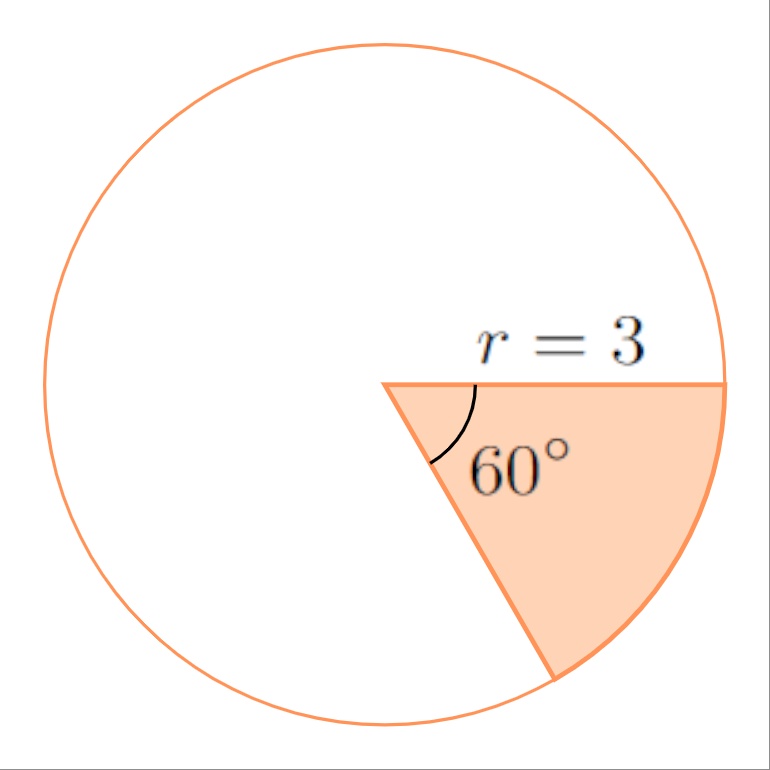
\includegraphics[width=0.6\linewidth]{mex_0061.png} $x=$\fillin[$38.11$][0cm]

            \begin{solutionbox}{4cm}
                \begin{align*}
                    c^2                & = a^2 + b^2  \\
                    44^2               & = 22^2 + x^2 \\
                    44^2 - 22^2        & = x^2        \\
                    \sqrt{44^2 - 22^2} & = x          \\
                    38.11              & \simeq x     \\
                \end{align*}
            \end{solutionbox}

            \part 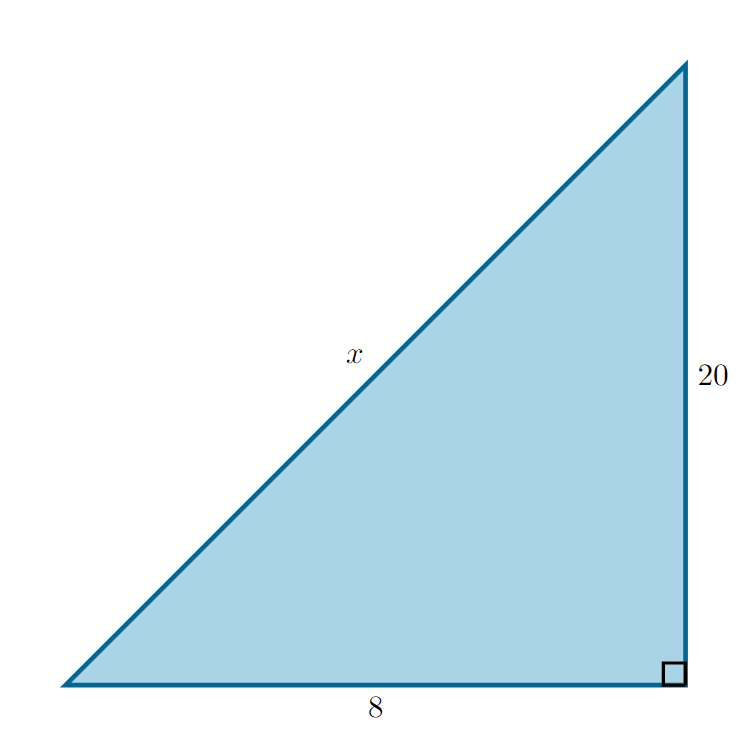
\includegraphics[width=0.6\linewidth]{mex_0057.png} $x=$\fillin[$21.54$][0cm]

            \begin{solutionbox}{4cm}
                \begin{align*}
                    c^2 & = a^2 + b^2  \\
                    x^2 & = 8^2 + 20^2 \\
                    x^2 & = 64 + 400   \\
                    x   & = \sqrt{464} \\
                    x   & \simeq 21.54 \\
                \end{align*}
            \end{solutionbox}
        \end{parts}
    \end{multicols}

    \question[] Encuentra el perímetro y el área de las siguientes figuras:

    \begin{multicols}{2}
        \begin{parts}
            \part  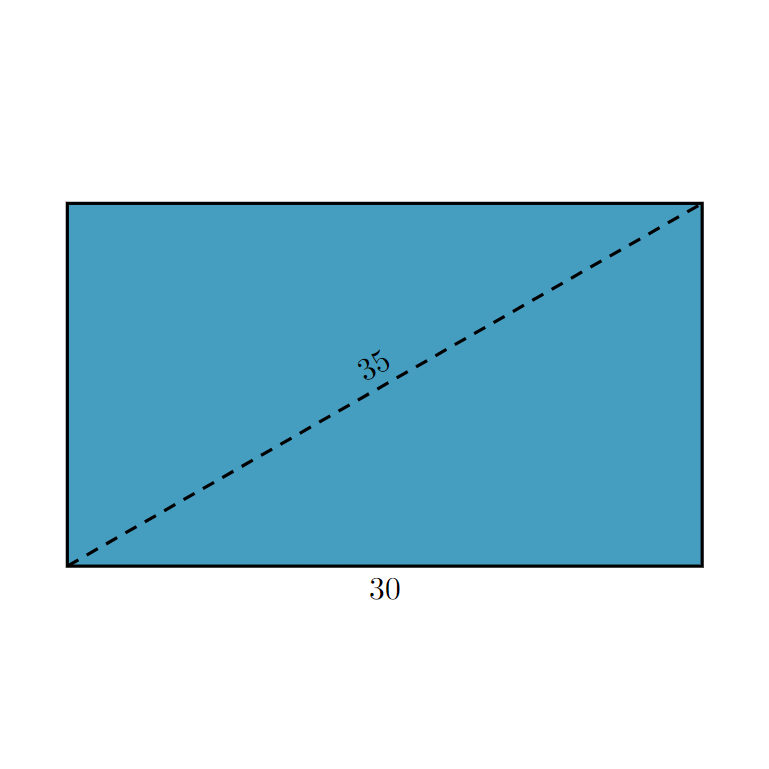
\includegraphics[width=0.8\linewidth]{mex_0066.png} $x=$\fillin[][0cm]

            \begin{solutionbox}{3cm}
            \end{solutionbox}

            \part 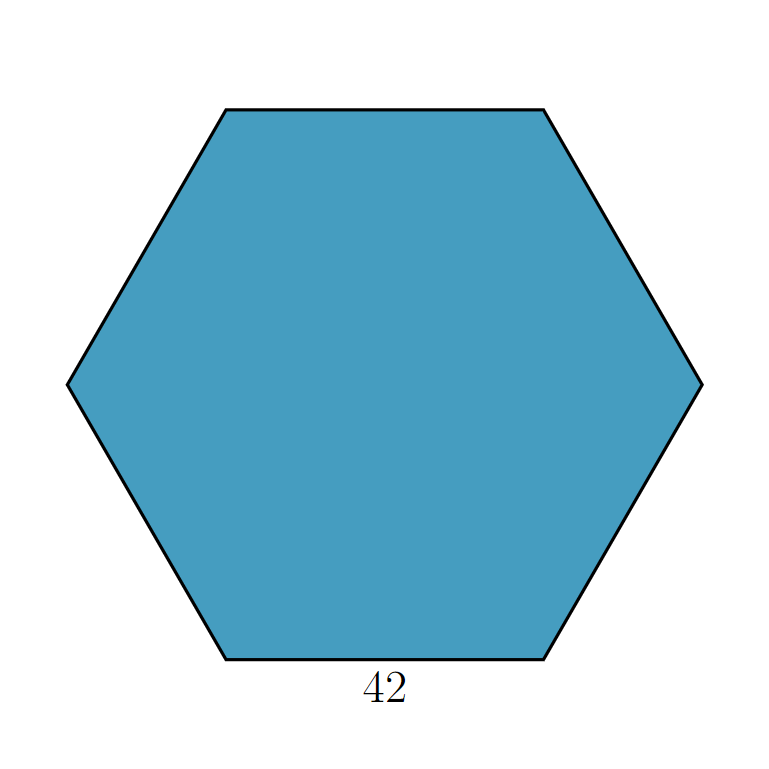
\includegraphics[width=0.8\linewidth]{mex_0067.png} $x=$\fillin[][0cm]

            \begin{solutionbox}{3cm}
            \end{solutionbox}
        \end{parts}
    \end{multicols}

    \question[] Resuelve los siguientes problemas:

    \begin{multicols}{2}
        \begin{parts}
            \part  Desde la ventana de una torre en la playa se ve un barco a 85 metros, cuando realmente se encuentra a 84 metros de la torre. ¿A qué altura está la ventana?

            \begin{solutionbox}{2cm}
                13
            \end{solutionbox}

            \part Calcula la altura de un triángulo isósceles cuya base mide 12 cm y sus lados iguales miden 25 cm.

            \begin{solutionbox}{2cm}
                24.26
            \end{solutionbox}
        \end{parts}
    \end{multicols}

    \question[] ¿Cuál es el cateto opuesto del ángulo A?
    \begin{multicols}{2}
        \begin{parts}
            \part $CO=$\fillin[$y$][0cm] 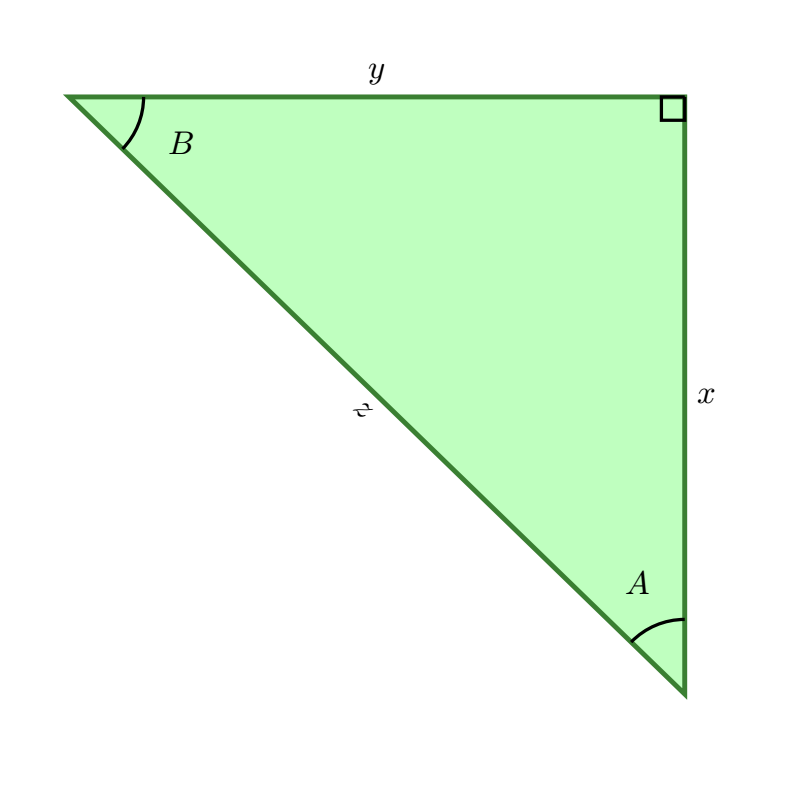
\includegraphics[width=0.8\linewidth]{mex_0075.png}
            \part $CO=$\fillin[$b$][0cm] 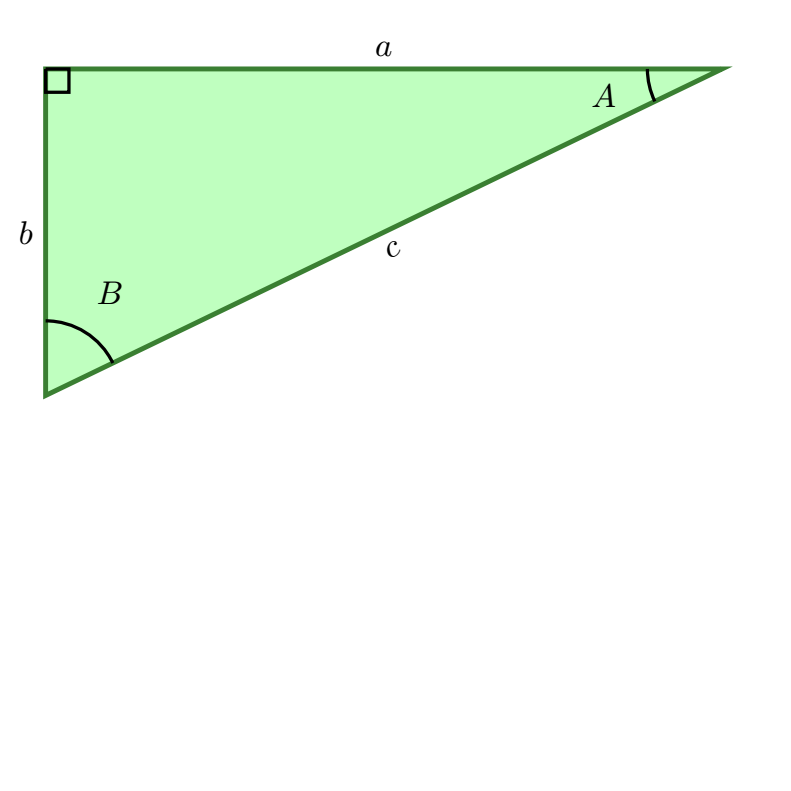
\includegraphics[width=0.65\linewidth]{mex_0072.png}
        \end{parts}
    \end{multicols}

    \question[] Con base en las siguientes imágenes, calcula lo que se te pide:

    \begin{multicols}{2}
        \begin{parts}
            \part {\Large 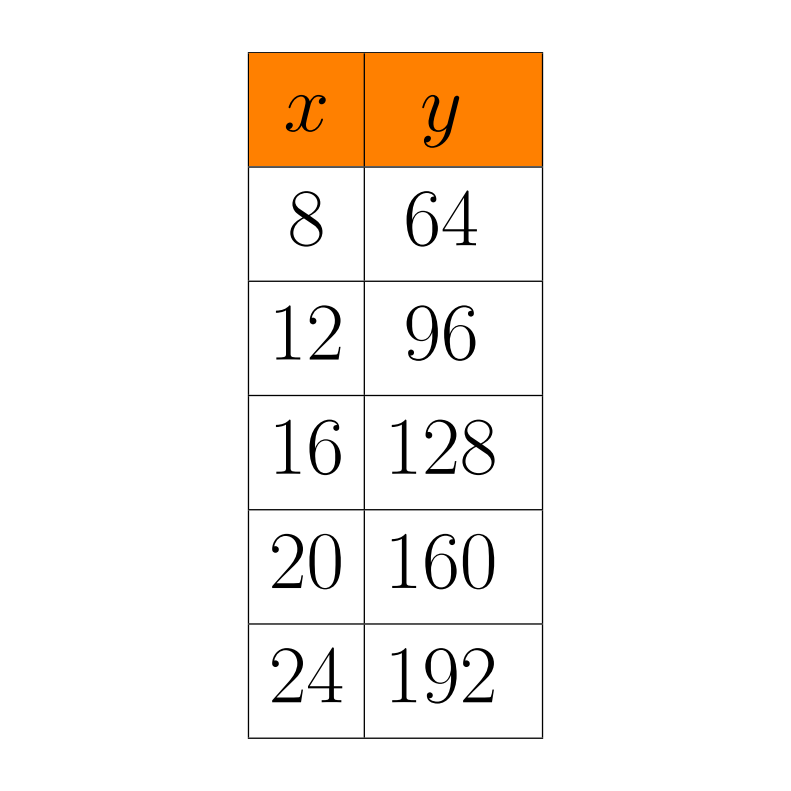
\includegraphics[width=0.75\linewidth]{mex_0081.png} \\ sen($B$)=\fillin[$0.24$][0cm]}
            \part {\Large 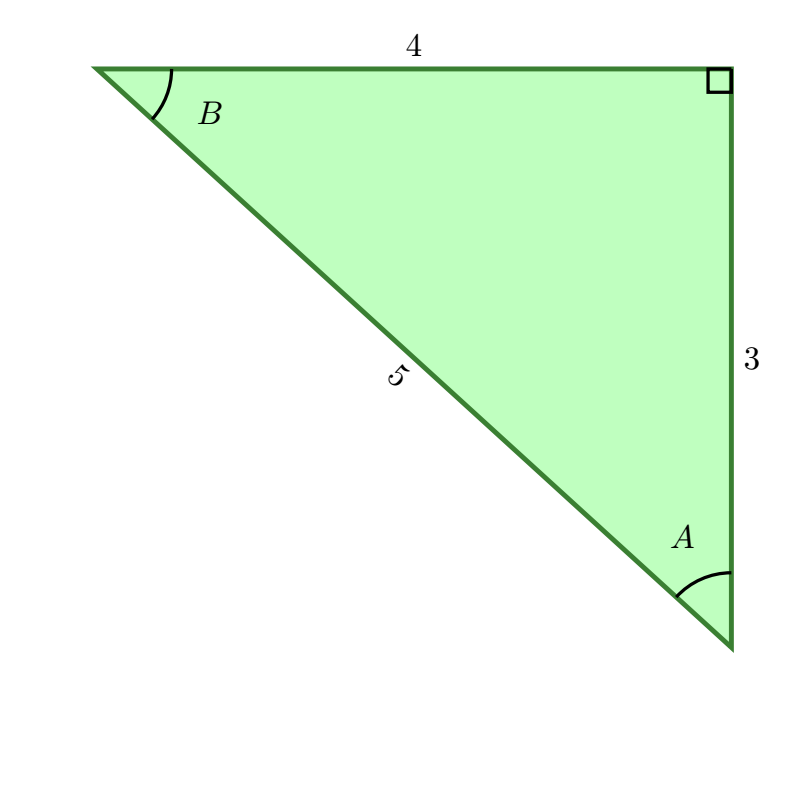
\includegraphics[width=0.75\linewidth]{mex_0082.png} \\ cos($A$)=\fillin[$0.60$][0cm]}
        \end{parts}
    \end{multicols}

    \question[] Usando la función trigonométrica correcta, encuentra el valor de los lados $x$, para cada uno de los siguientes ejercicios:

    \begin{multicols}{2}
        \begin{parts}
            \part  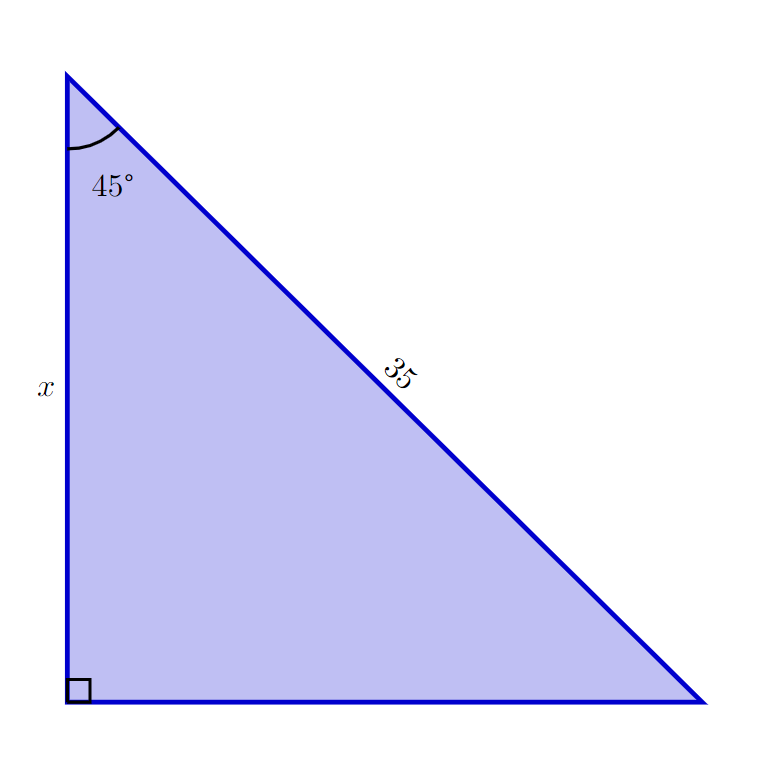
\includegraphics[width=0.75\linewidth]{mex_0091.png} \\ $x=$\fillin[$37.08$][0cm]
            \part 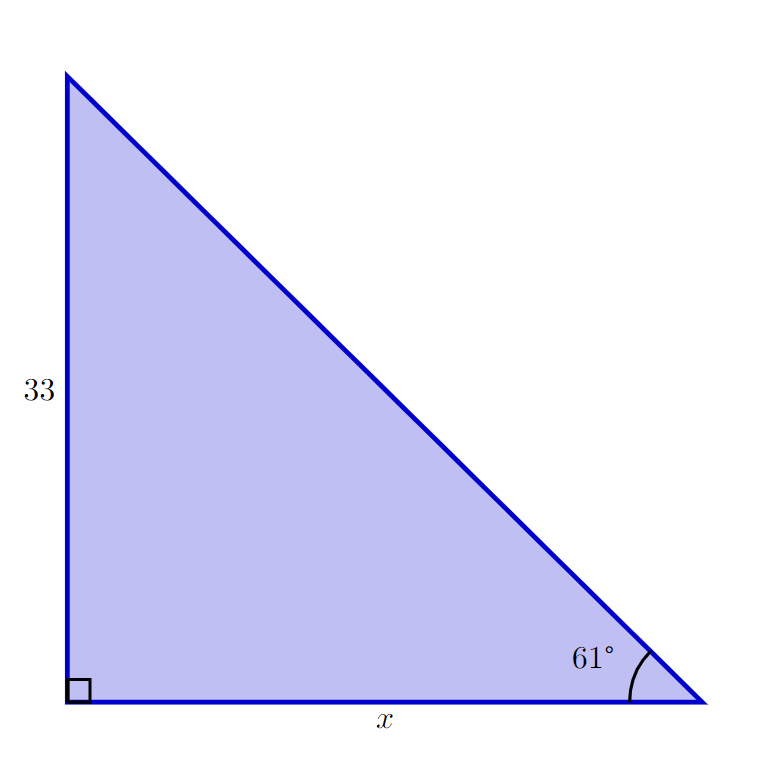
\includegraphics[width=0.75\linewidth]{mex_0092.png}  \\ $x=$\fillin[$24.84$][0cm]
        \end{parts}
    \end{multicols}

    \question[] Usando la función trigonométrica correcta, encuentra el valor de los ángulos $x$, para cada uno de los siguientes ejercicios:

    \begin{multicols}{2}
        \begin{parts}
            \part  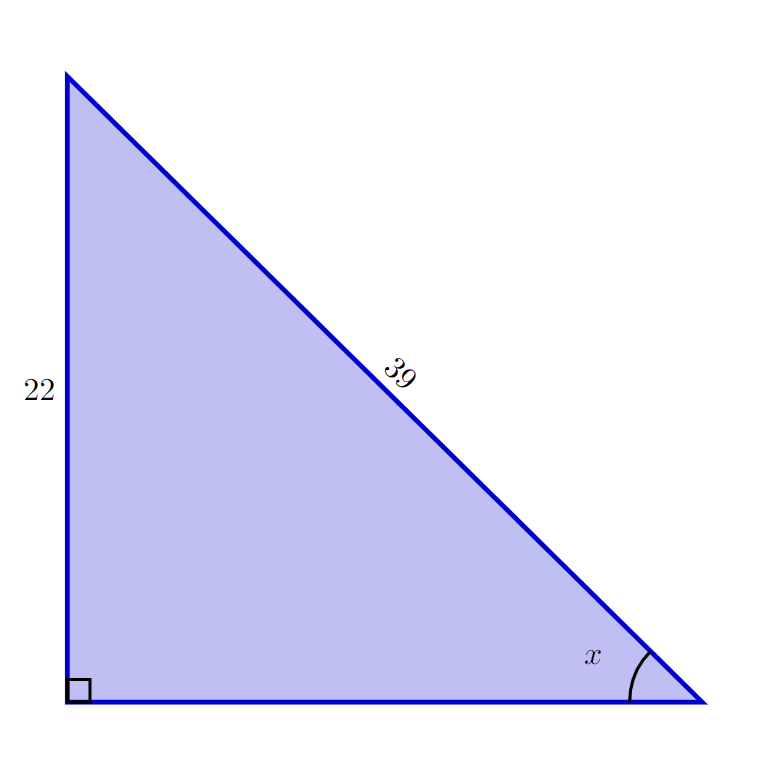
\includegraphics[width=0.75\linewidth]{mex_0096.png} \\ $x=$\fillin[$34.33$][0cm]
            \part 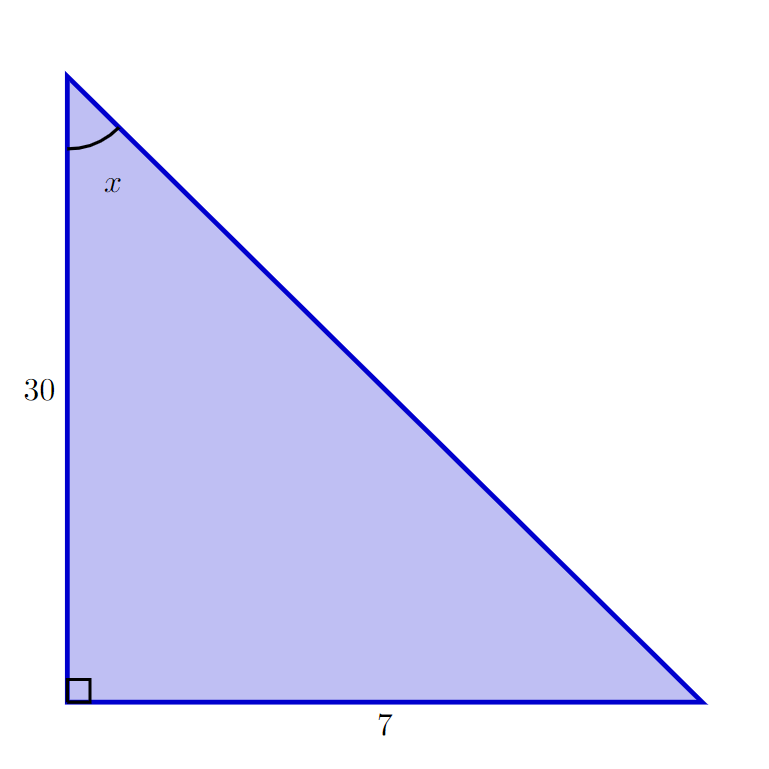
\includegraphics[width=0.75\linewidth]{mex_0097.png}  \\ $x=$\fillin[$13.13$][0cm]
        \end{parts}
    \end{multicols}

    \question[] Resuelve los siguientes problemas:

    \begin{multicols}{2}
        \begin{parts}
            \part  El piloto de un avión debe aproximarse a la pista de aterrizaje con un ángulo de 7° con respecto a la horizontal. Si vuela a una altura de 8,000 metros, ¿a qué distancia de la pista debe iniciar su descenso?

            \begin{solutionbox}{2cm}
                65154.77
            \end{solutionbox}

            \part El sonar de un barco de salvamiento localiza los restos de un naufragio en un ángulo de depresión de 40°. Un buzo es bajado 40 metros hasta el fondo del mar, ¿cuánto necesita avanzar el buzo por el fondo para encontrar los restos del naufragio?

            \begin{solutionbox}{2cm}
                47.67
            \end{solutionbox}
        \end{parts}
    \end{multicols}

    \question[]

    \question[]


\end{questions}
\end{document}